\section{Projeto de Controle}

\subsection{Modelagem Térmica do Sistema}

O primeiro passo para a implementação do controle de temperatura da fermentação é a modelagem térmica do processo. Nota-se que essa modelagem é bastante complexa pois envolve diversos coeficientes térmicos desconhecidos, devido a composição heterogênea do Mosto com Leveduras. 


A fermentação ocorre na maior  parte das receitas em temperaturas de 14°C até 20°C,  temperaturas muitas vezes inferiores à temperatura do ambiente. Sendo assim, existe a necessidade de criar um sistema que troque calor com o mosto e leveduras mantendo um gradiente de temperatura entre o fermentador e o ambiente constante conforme configuração do usuário. 


Para isso acontecer durante o processo, o calor retirado pela refrigeração deve ser o mesmo que o gerado pela convecção com o ambiente e pelo próprio processo de fermentação, que é exotérmico. 


É possível dividir essa modelagem em três partes:  
\begin{enumerate}
    \item Determinação da quantidade de calor trocada pelo fermentador e o ambiente.
    \item Determinação da quantidade de calor ganha no processo de fermentação.
    \item Projeto e modelagem do dispositivo de troca de calor.
\end{enumerate}
    

É importante destacar que o dispositivo irá ter duas funções: a primeira será manter a temperatura do líquido fermentado; a segunda será levar o líquido até determinada temperatura. Ambas as funcionalidades envolvem a capacidade do dispositivo de retirar ou fornecer calor do sistema de forma eficiente e constante. 


\subsection{Transferência de Calor entre Ar e Fermentador}

Nessa modelagem, serão analisados os seguintes elementos: 
\begin{itemize}
    \item Mosto e Leveduras 
    \item Tanque de Fermentação 
    \item Manta Térmica 
\end{itemize}

Nessa dinâmica, considerando que o fermentador vai operar na maior parte do tempo em temperaturas inferiores às do ambiente, o calor vai fazer o seguinte caminho:

\begin{center}
    \(Ambiente \longrightarrow Manta\;t\acute{e}rmica \longrightarrow Fermentador \longrightarrow Mosto\;e\;leveduras\)
\end{center}
    


Sendo assim, é possível obter o calor ganho por convecção para cada 1°C de diferença de temperatura entre o fermentador e o ambiente


Algumas hipóteses foram adotadas visando simplificar o problema: 

\begin{enumerate}
    \item O gradiente de temperatura no interior do Mosto + Leveduras é desprezível; 
    \item O coeficiente de troca de calor por convecção entre o Mosto + leveduras e o tanque é elevados o bastante para que não sejam observadas diferenças de temperatura entre esses elementos; 
    \item O regime é permanente e as propriedades são constantes 
    \item A condução é unidimensional no plano X
    \item A transferência de calor por radiação é desprezível nas superfícies 
    \item Resistências de contato desprezíveis.
\end{enumerate}


As hipóteses 1, 2, 3  podem ser adotadas devido ao horizonte de tempo da fermentação, no qual é necessário manter a mesma temperatura durante dias. As hipóteses 4, 5 e 6 foram adotadas com a intenção de simplificar o problema. A figura \ref{fig:fermentador_controle} exemplifica esse problema e a figura \ref{fig:fermentador_circuito} demonstra o circuito elétrico equivalente, cuja legenda se encontra na tabela \ref{tab:variaveis_circuito}.

\begin{figure}[h]
    \centering
    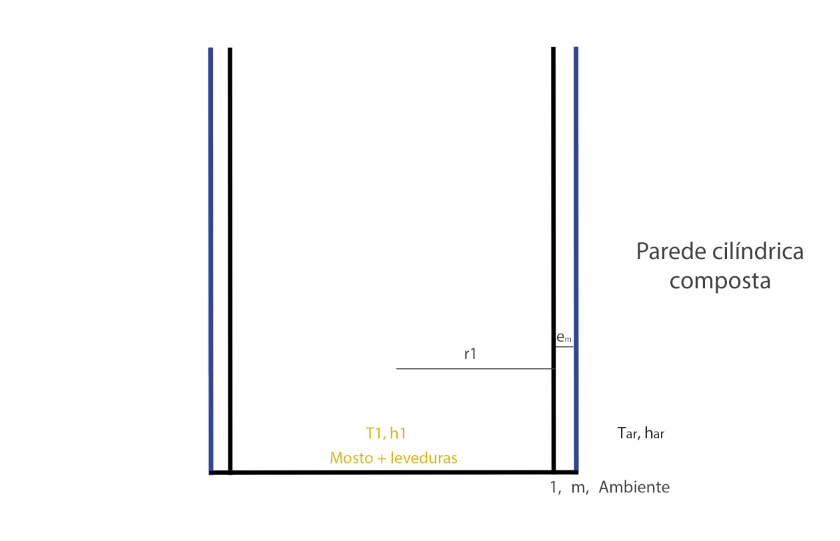
\includegraphics[scale=0.35]{figuras/projeto/controle/fermentador_controle.png}
    \caption{Desenho do problema de troca de calor entre o ambiente e fermentador}
    \label{fig:fermentador_controle}
\end{figure}

\begin{figure}[h]
    \centering
    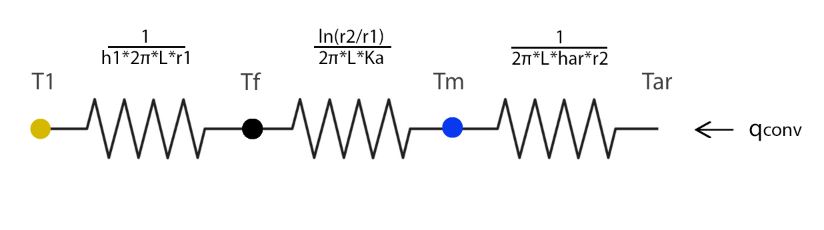
\includegraphics[scale=0.40]{figuras/projeto/controle/fermentador_circuito.png}
    \caption{Circuito elétrico equivalente ao problema de troca de calor entre ambiente e fermentador}
    \label{fig:fermentador_circuito}
\end{figure}

\begin{table}
    \begin{center}
        \begin{tabular}{ |c|c| } 
            \hline
            Variável   &  Descrição  \\
            \hline
            \(r_1\)   &  raio do fermentador  \\
            \hline
            \(e_m\) &  espessura da manta \\
            \hline
            \(r_2\)   &  em + r1   \\
            \hline
            \(T_1\)  &  temperatura desejada para a fermentação, \\
            \hline
            \(T_{ar}\) &  temperatura ambiente  \\
            \hline
            \(L\)    &  Altura do fermentador  \\
            \hline
            \(h_1\)  &  coeficiente de transferência térmica do Mosto + Leveduras  \\
            \hline
            \(h_{ar}\) &  coeficiente de transferência térmica do ar \\
            \hline
            \(K_a\) & Condutividade térmica da manta  \\
            \hline
            \(q_{conv}\) & quantidade de calor perdida por convecção (J/kg) \\
            \hline
        \end{tabular}
        \caption{\label{tab:variaveis_circuito}Descrição das variáveis do circuito elétrico equivalente da figura \ref{fig:fermentador_circuito}.}
    \end{center}
\end{table}

Sendo:

\begin{equation}
    q = \dfrac{T_1 - T_2}{R_{12}}
\end{equation}


A equação \ref{eq:circuito} define a quantidade de calor recebida pelo mosto e leveduras devido a convecção natural:  


\begin{equation}
    q_{conv} = (T_{ar} - T_1) \cdot (2 \pi L) \cdot (\dfrac{h_1 \cdot h_{ar} \cdot K_a \cdot r_2 \cdot r_1}{k_a \cdot h_{ar} \cdot r_2 + \ln(r_2/r_1) \cdot h_1 \cdot h_{ar} \cdot r_2 \cdot r_1 + h_1 \cdot k_a \cdot r_1})
    \label{eq:circuito}
\end{equation}

\subsection{Geração de Calor na Fermentação}

O processo de fermentação é exotérmico, logo existe a produção de calor. Segundo Munroe (\citeonline{FermentationMunroe}), é estimada a produção de 585,76 kJ por Kg de mosto. Como a maior parte do calor é gerado durante a fase de crescimento exponencial da fermentação, que acontece durante os 4 primeiros dias, iremos estimar que ocorre a troca de \(587,76 * 10^3 / (4*24*60*60)W = 1,7 W\) por kg de mosto durante os 4 primeiros dias de fermentação.   

\subsection{Dispositivo para Troca de Calor}

Um dos maiores desafios do projeto é criar um sistema que consiga trocar calor de forma eficiente, não seja intrusivo e consiga ser simples o suficiente para ser utilizado por um hobbysta. Conforme anteriormente especificado, a ideia é utilizar placas de peltier para realizar essa troca. A maior vantagem do uso dessas placas é a possibilidade de controlar o calor associado proporcionalmente a quantidade de corrente fornecida ao módulo, através da seguinte equação \ref{eq:qp}.

\begin{equation}
    Q_P = \pi \cdot 1
    \label{eq:qp}
\end{equation}

Possibilitando assim o uso de um circuito junto com o microcontrolador para o controle de temperatura. 
O sistema será composto por um dissipador de calor e um dissipador de calor e uma ventoinha na face quente (figura \ref{fig:cooler}). Dessa forma podemos otimizar a expulsão de calor do dispositivo. E uma haste de cobre (figura \ref{fig:haste_cobre}) ligado no lado frio, o metal é considerado um bom condutor térmico e servirá como condutor de calor entre a o fermentador e o módulo de Peltier. Essa abordagem foi inspirada no aparelho homebrew citado anteriormente. 

\begin{figure}[h]
    \centering
    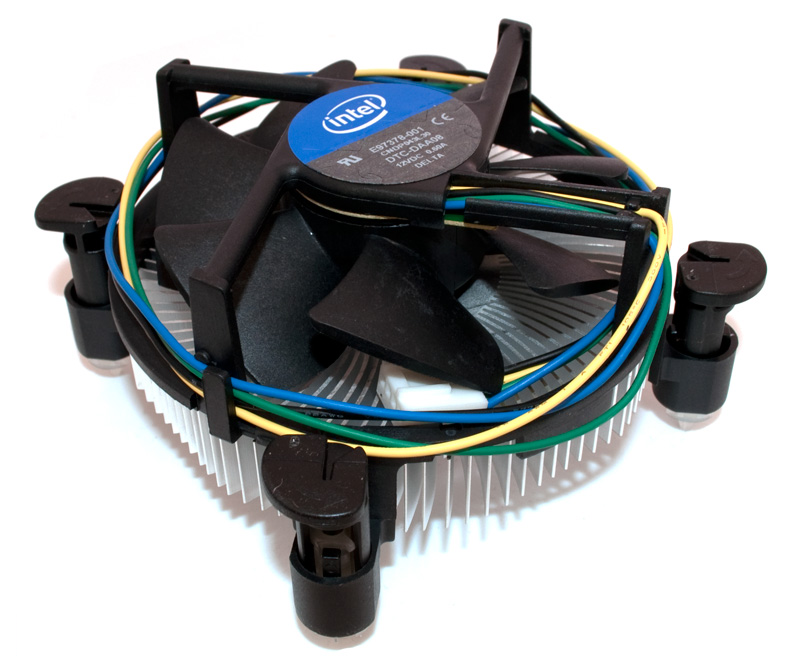
\includegraphics[scale=0.20]{figuras/projeto/controle/cooler.png}
    \caption{Dissipador de calor e ventoinha, modelo utilizado em CPU.}
    \label{fig:cooler}
\end{figure}


\begin{figure}[h]
    \centering
    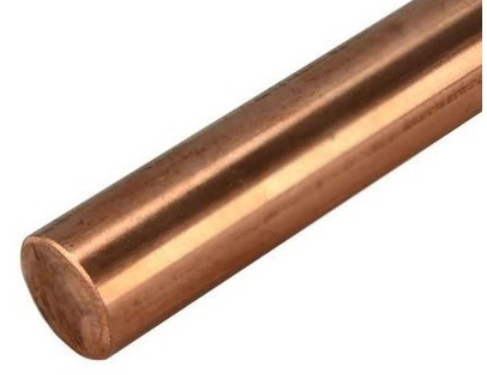
\includegraphics[scale=0.30]{figuras/projeto/controle/haste.png}
    \caption{Haste de cobre.}
    \label{fig:haste_cobre}
\end{figure}
